\subsubsection{VBO behavior}\label{sssec:VBO_behavior}
This section focusses on the output of the source follower that is directly connected to the output of the high voltage transistor connected to the input of the ROIC. The setup is identical to \cref{sssec:standard_behavior}, but the time scale is different to oberve the slower behavior of VBO.

\Cref{fig:vbo_slopes} shows the time against voltage plot. This are a couple of important observations that can be made from these plots. First and foremost: the behavior of the VBO is almost not affected by the capacitance. There is a difference however, in that the VBO starts rising as the OUT reaches zero. This means that the VBO for $450\,fF$ is slightly delayed when compared to $50\,fF$. It is also intersting to observe that VBO never increases above $3.8\,V$. This behavior is most likely due to the functioning of the voltage limiter that will be ivestigated later on. Finally one can observe that for very low currents, VBO does not reach $2.6\,V$. The reason for this is that the input reaches the voltage level of the power supply before the current limiter kicks in.


\begin{figure}[h]
    \centering
    \begin{subfigure}[b]{0.475\textwidth}
        \centering
        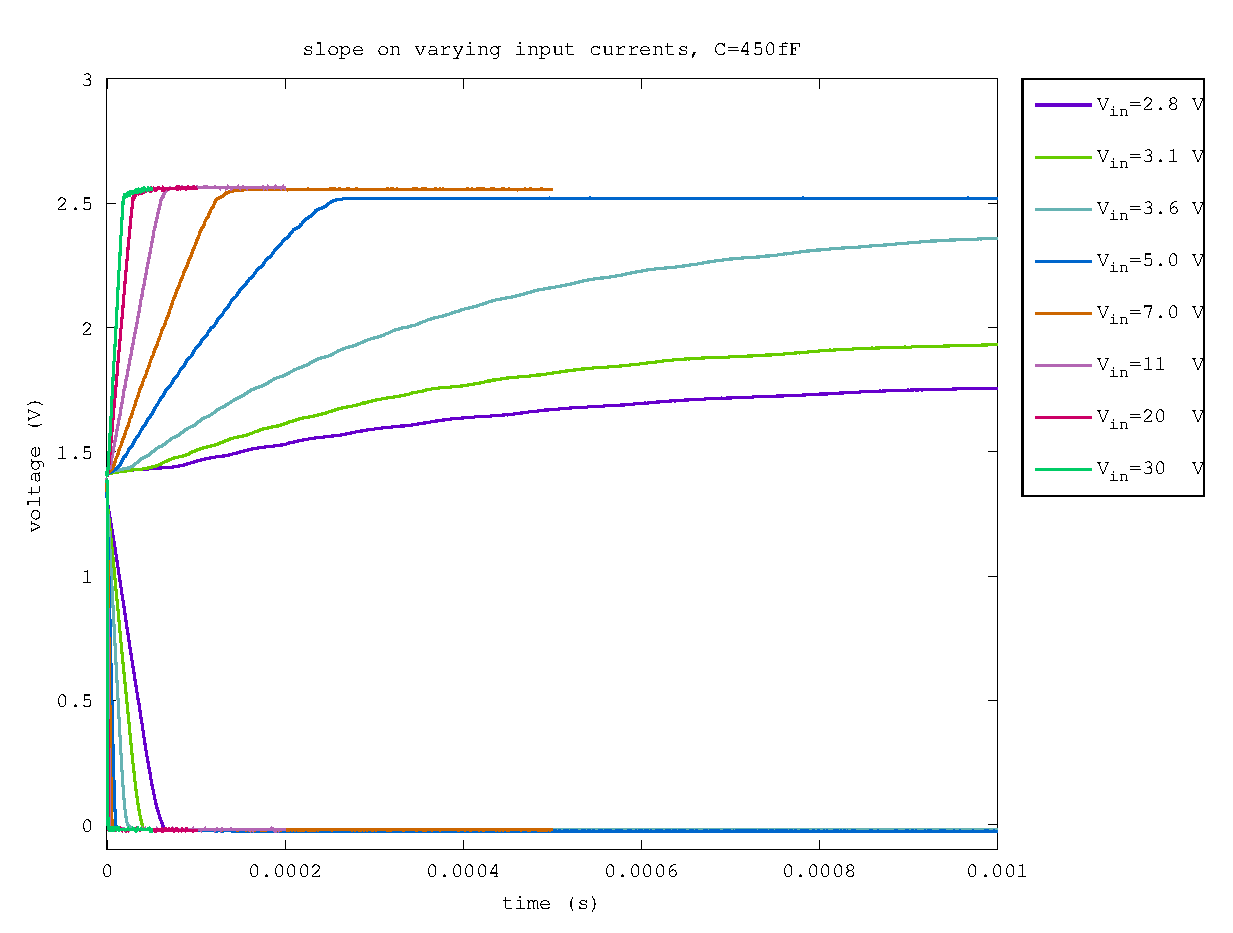
\includegraphics[width=\textwidth]{fig/vbo_slope_450fF.eps}
        \caption[Network2]%
        {$C0$}    
        \label{fig:vbo_slopes_450fF}
    \end{subfigure}
    \hfill
    \begin{subfigure}[b]{0.475\textwidth}  
        \centering 
        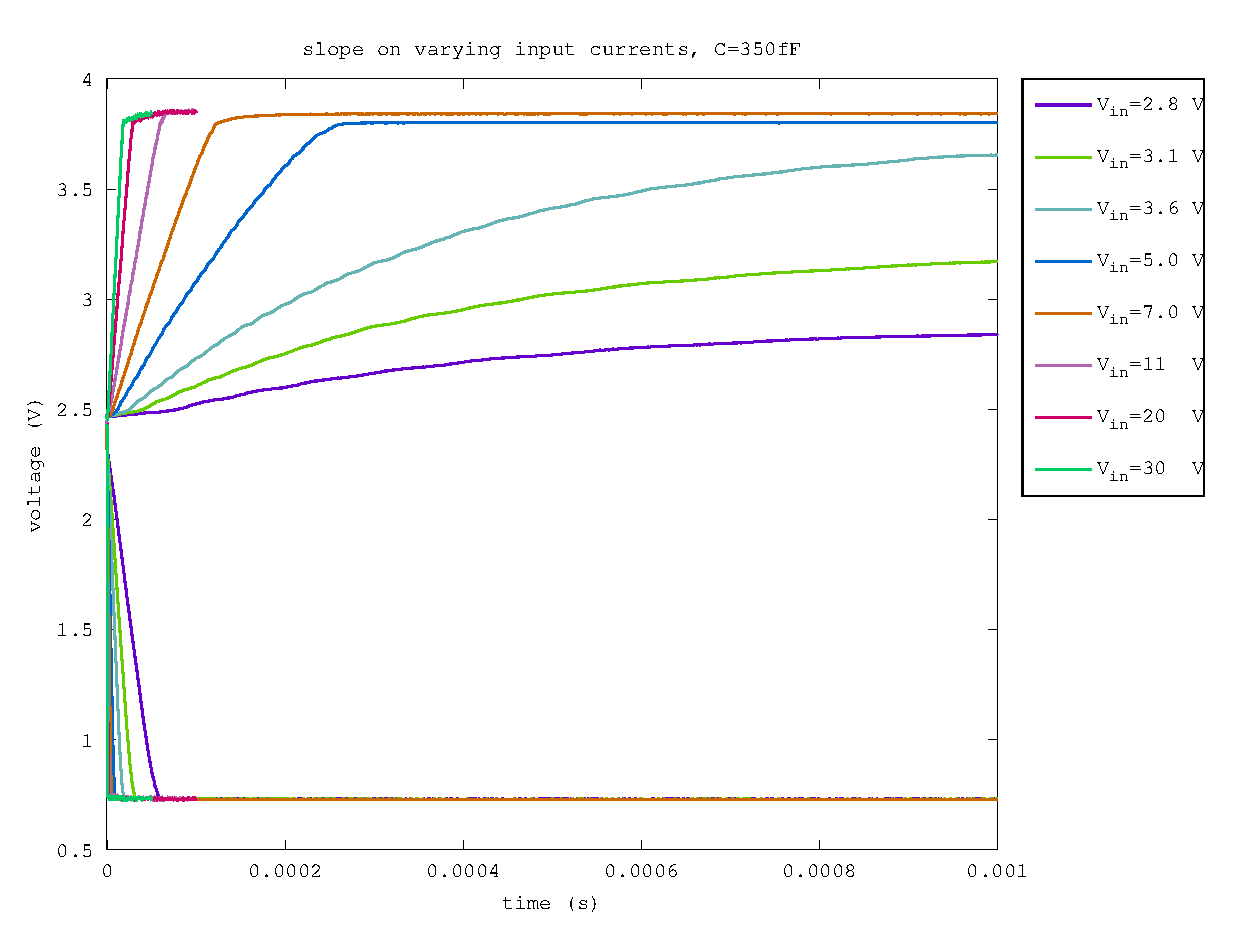
\includegraphics[width=\textwidth]{fig/vbo_slope_350fF.eps}
        \caption {$C1$}    
        \label{fig:vbo_slopes_350fF}
    \end{subfigure}
    \vskip\baselineskip
    \begin{subfigure}[b]{0.475\textwidth}   
        \centering 
        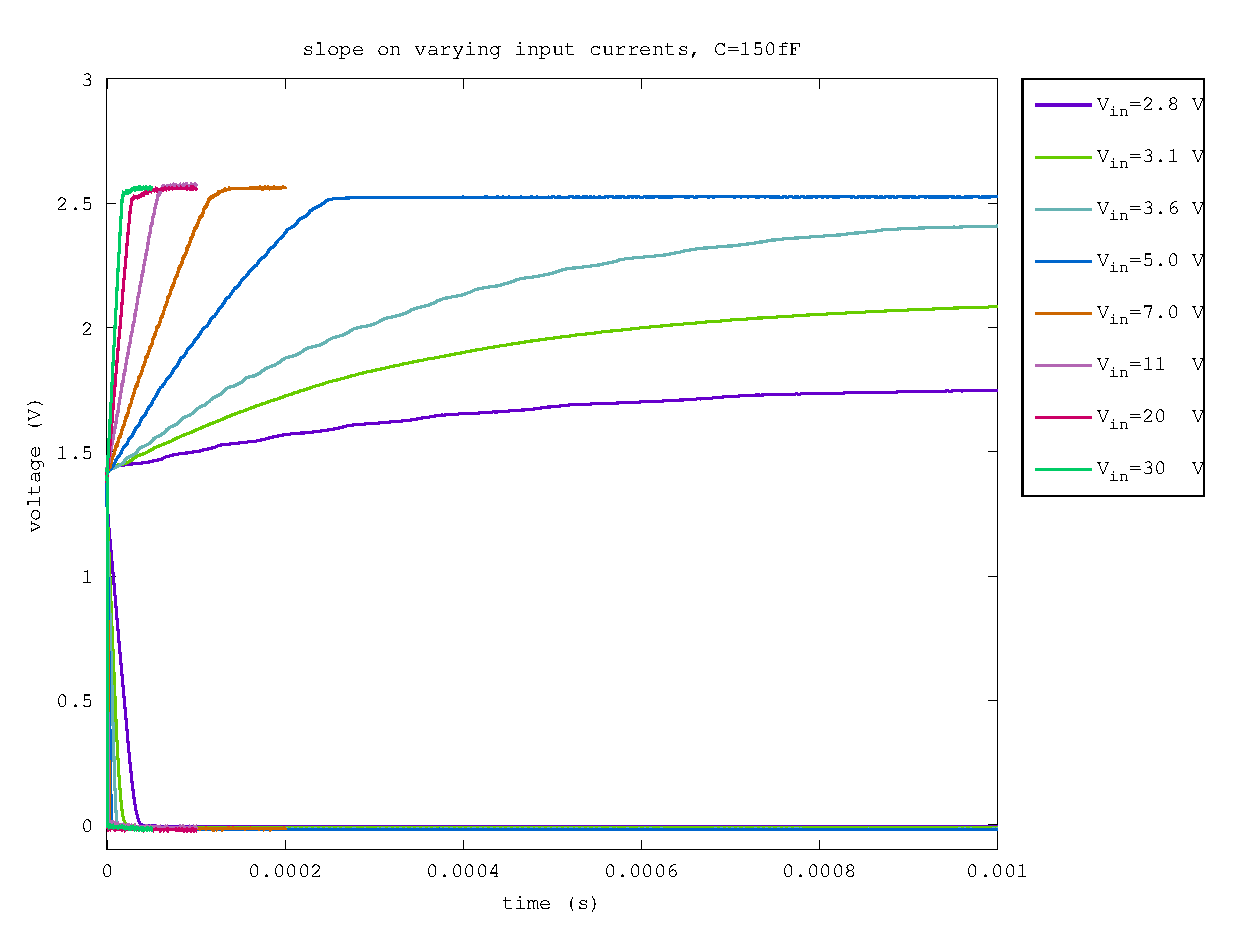
\includegraphics[width=\textwidth]{fig/vbo_slope_150fF.eps}
        \caption{$C2$}    
        \label{fig:vbo_slopes_150fF}
    \end{subfigure}
    \quad
    \begin{subfigure}[b]{0.475\textwidth}   
        \centering 
        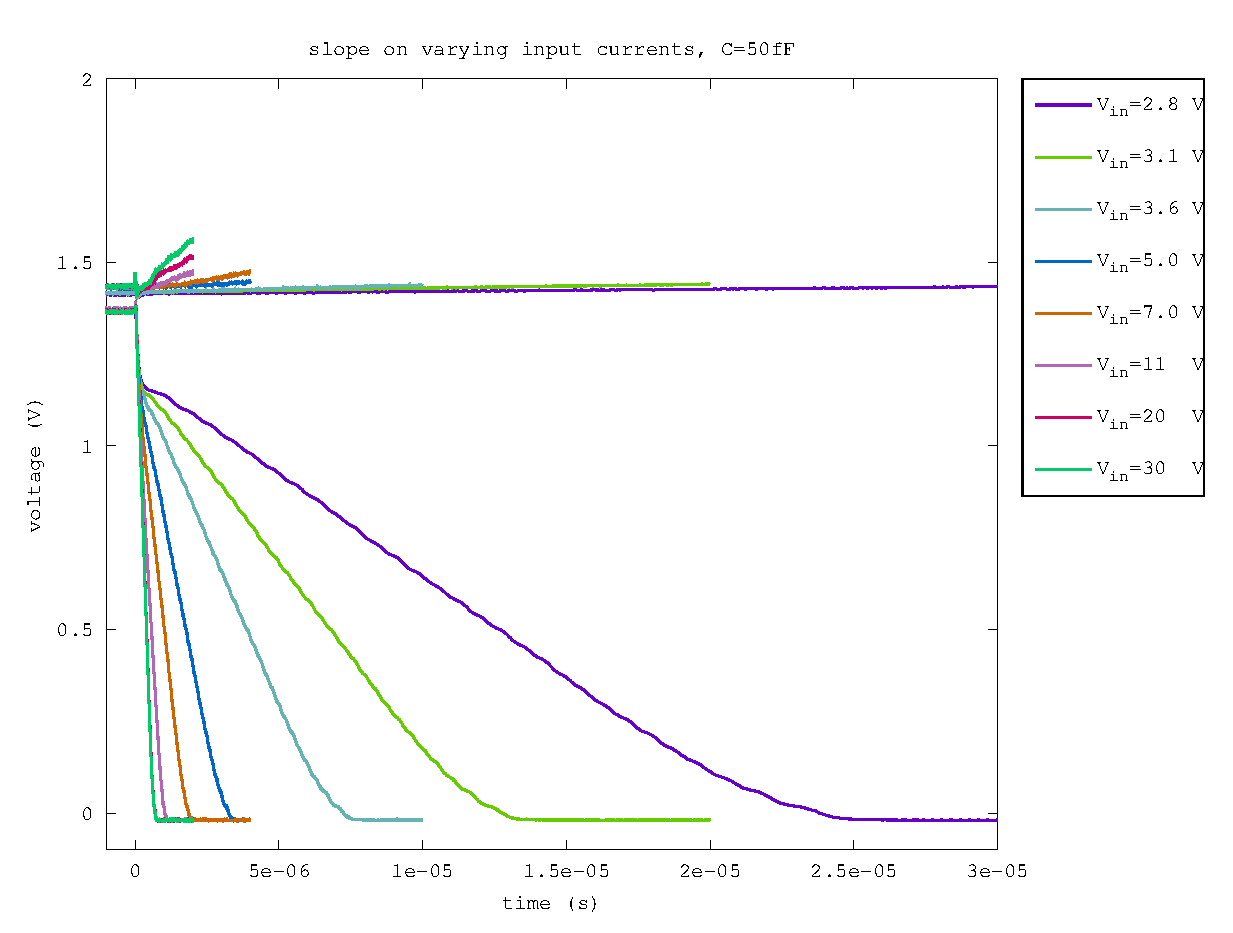
\includegraphics[width=\textwidth]{fig/vbo_slope_50fF.eps}
        \caption{$C3$}    
        \label{fig:vbo_slopes_50fF}
    \end{subfigure}
    \caption{Expected versus measured charge up times for different input voltages. The input voltage is connected to the input through a resistor of $20\,M\Omega$}
    \label{fig:vbo_slopes}
\end{figure}

\Cref{fig:vbo_charges} shows the plots of voltage against charge. One can observe that increasing the current causes the behavior to converge to a line with a linear slope that is constant with Q, and a saturation at $3.8\,V$. 

\begin{figure}[h]
    \centering
    \begin{subfigure}[b]{0.475\textwidth}
        \centering
        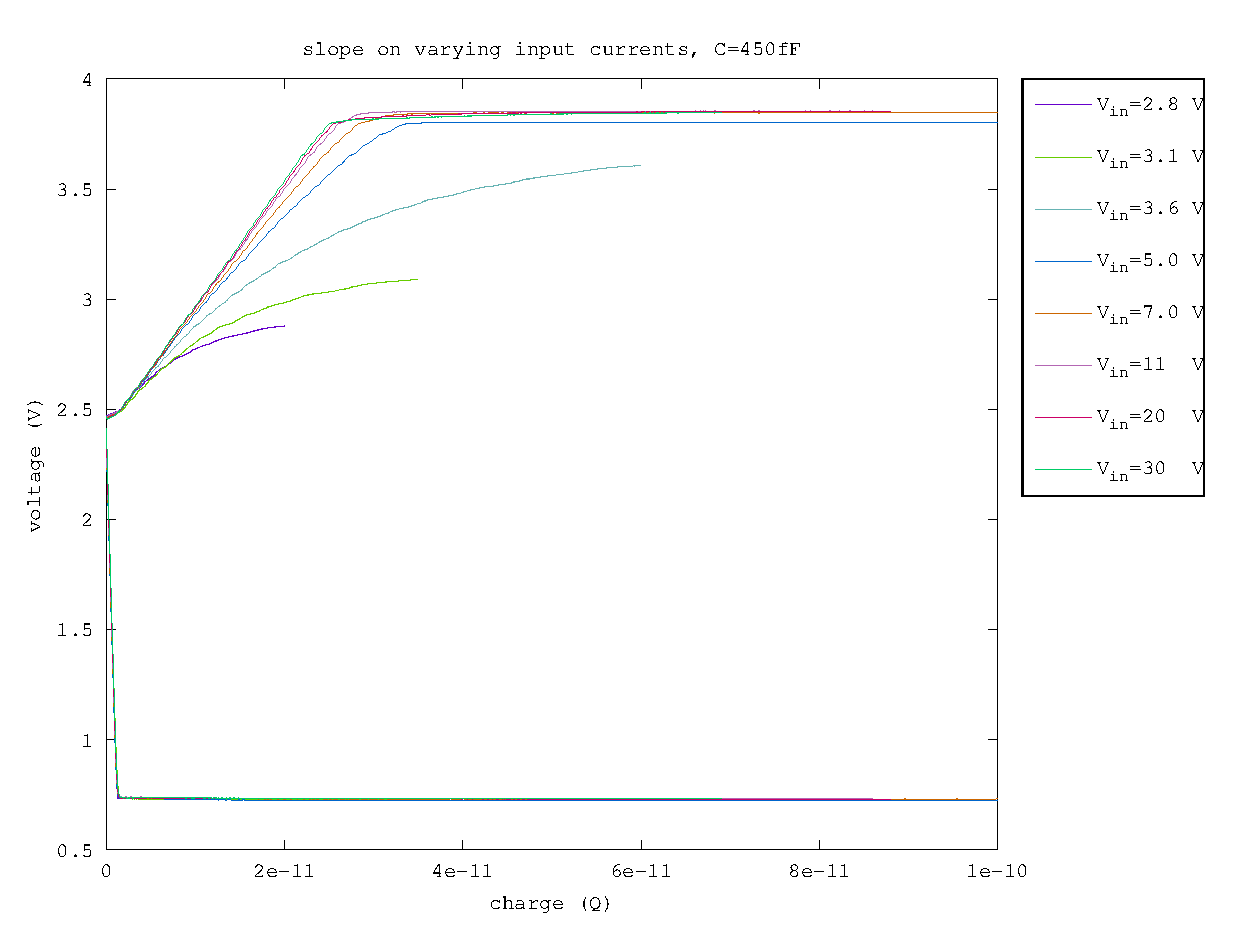
\includegraphics[width=\textwidth]{fig/vbo_charge_450fF.eps}
        \caption[Network2]%
        {$C0$}    
        \label{fig:vbo_charges_450fF}
    \end{subfigure}
    \hfill
    \begin{subfigure}[b]{0.475\textwidth}  
        \centering 
        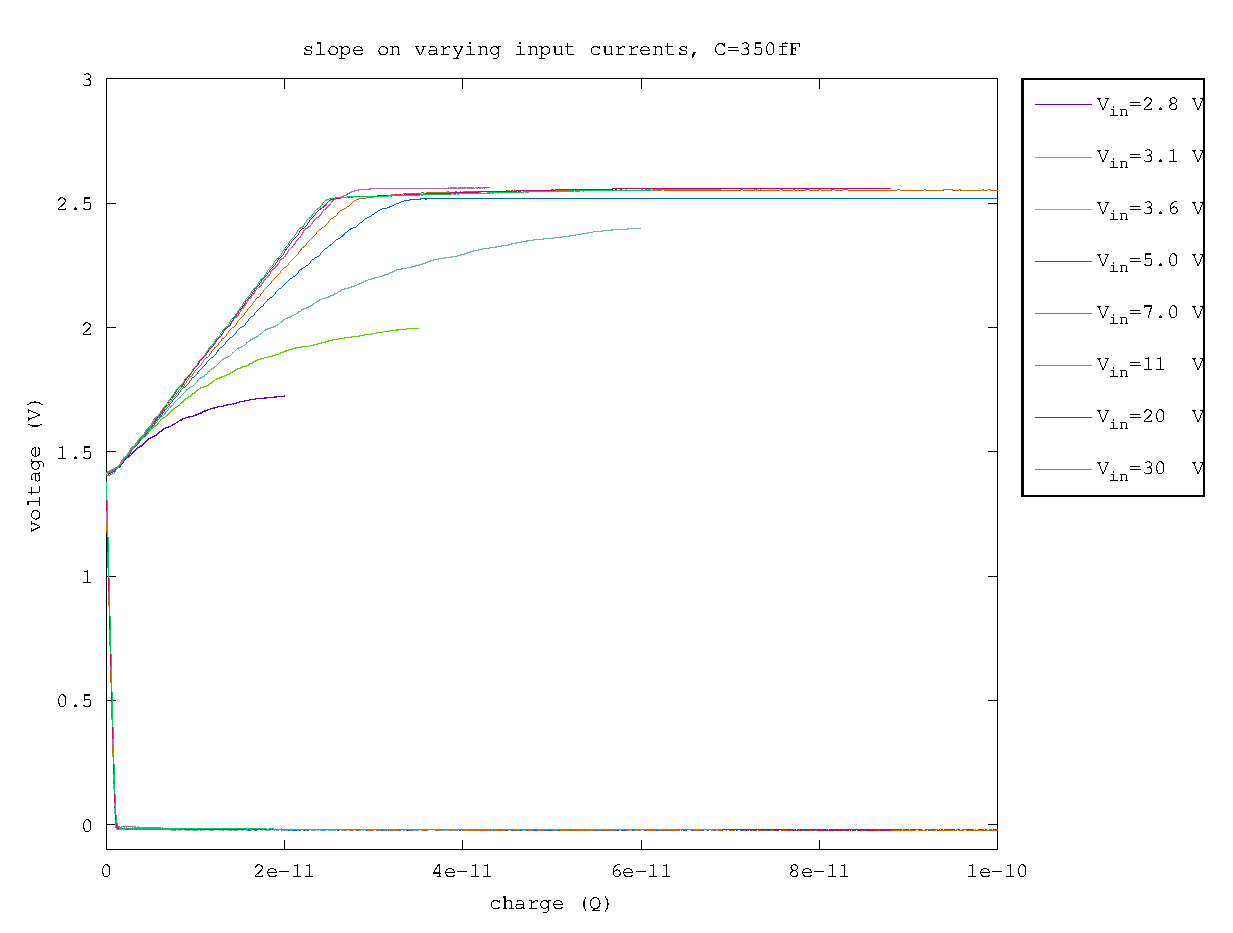
\includegraphics[width=\textwidth]{fig/vbo_charge_350fF.eps}
        \caption{$C1$}    
        \label{fig:vbo_charges_350fF}
    \end{subfigure}
    \vskip\baselineskip
    \begin{subfigure}[b]{0.475\textwidth}   
        \centering 
        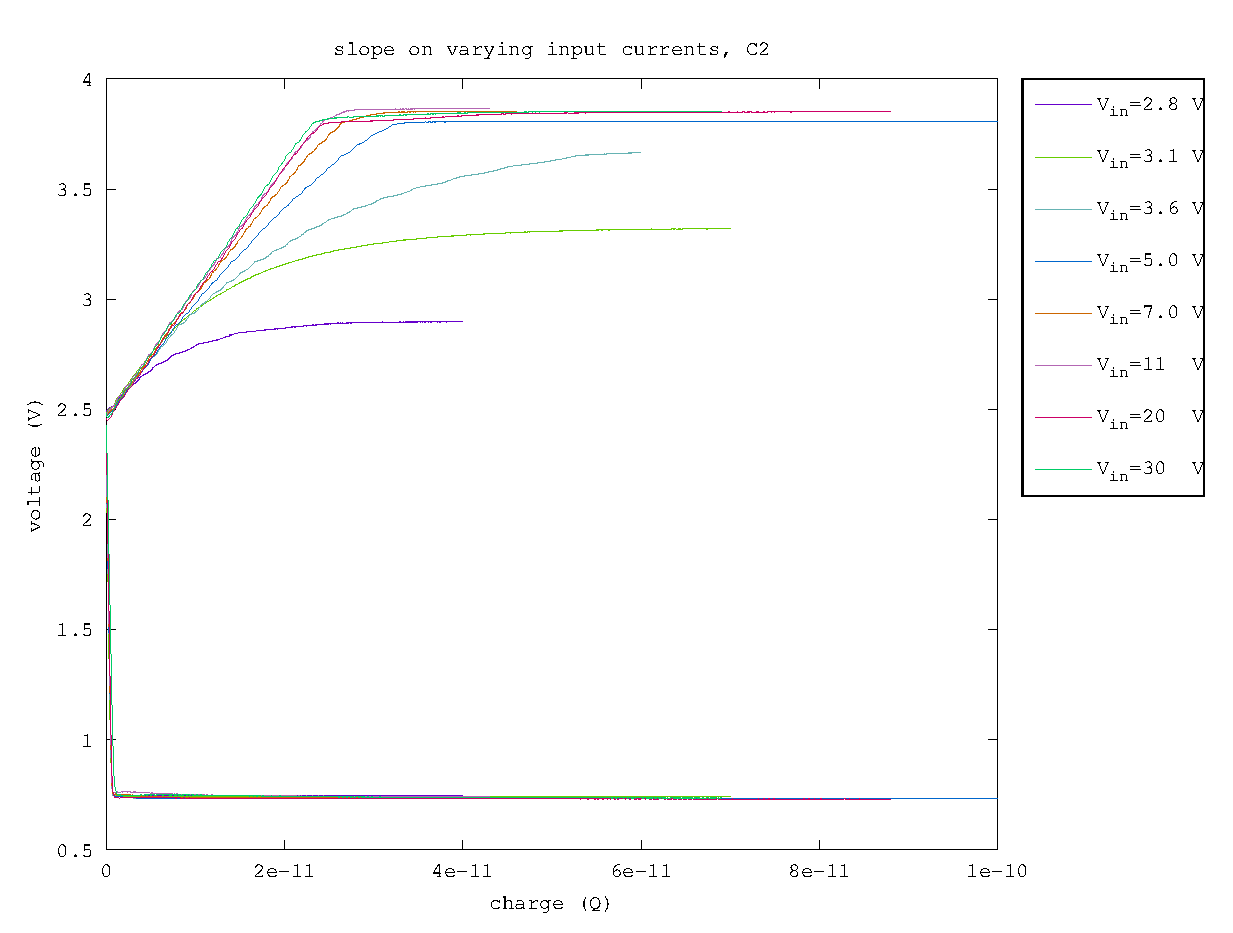
\includegraphics[width=\textwidth]{fig/vbo_charge_150fF.eps}
        \caption{$C2$}    
        \label{fig:vbo_charges_150fF}
    \end{subfigure}
    \quad
    \begin{subfigure}[b]{0.475\textwidth}   
        \centering 
        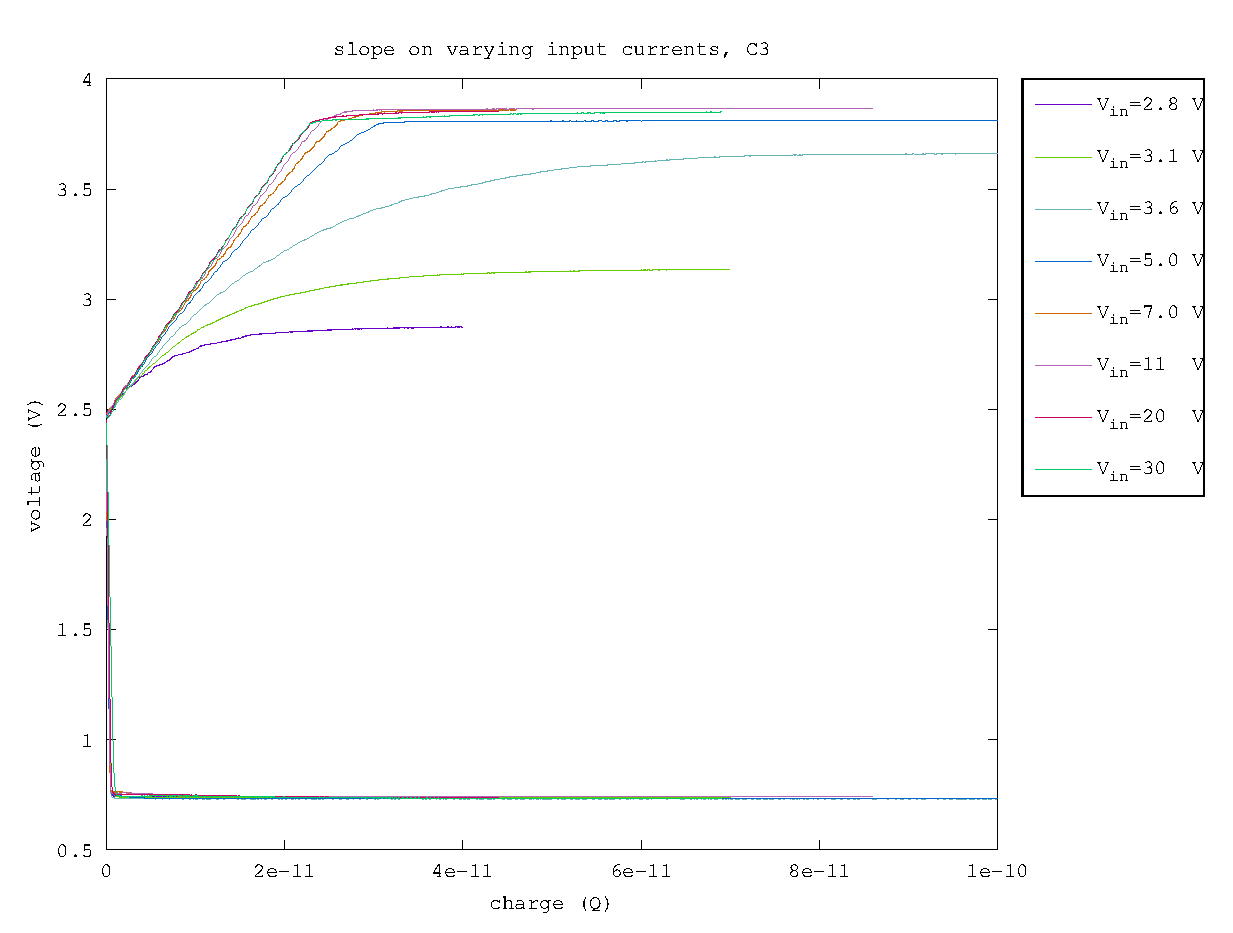
\includegraphics[width=\textwidth]{fig/vbo_charge_50fF.eps}
        \caption {$C3$}    
        \label{fig:vbo_charges_50fF}
    \end{subfigure}
    \caption{This plot is showing charge versus voltage}
    \label{fig:vbo_charges}
\end{figure}

\Cref{fig:vbo_d_slopes} shows $\delta V/\delta Q$ for the VBO. The main observation one can make fromthese plots is that the behavior of VBO is almost entirely unaffected by the integration capacitance.


\begin{figure}[h]
    \centering
    \begin{subfigure}[b]{0.475\textwidth}
        \centering
        \includegraphics[width=\textwidth]{fig/vbo_d_slope_450fF.eps}
        \caption[Network2]%
        {$C0$}    
        \label{fig:vbo_d_slopes_450fF}
    \end{subfigure}
    \hfill
    \begin{subfigure}[b]{0.475\textwidth}  
        \centering 
        \includegraphics[width=\textwidth]{fig/vbo_d_slope_350fF.eps}
        \caption  {$C1$}    
        \label{fig:vbo_d_slopes_350fF}
    \end{subfigure}
    \vskip\baselineskip
    \begin{subfigure}[b]{0.475\textwidth}   
        \centering 
        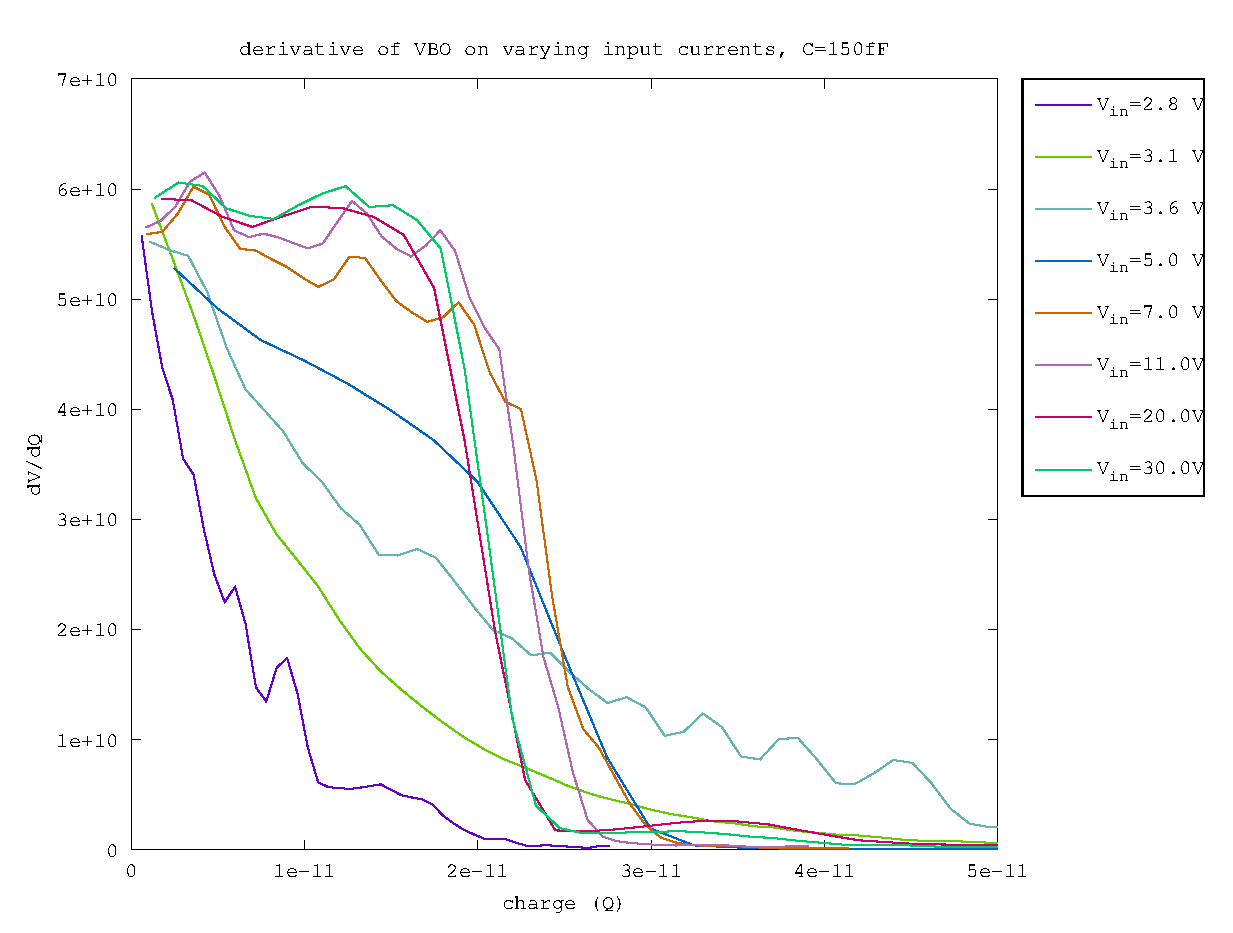
\includegraphics[width=\textwidth]{fig/vbo_d_slope_150fF.eps}
        \caption {$C2$}    
        \label{fig:vbo_d_slopes_150fF}
    \end{subfigure}
    \quad
    \begin{subfigure}[b]{0.475\textwidth}   
        \centering 
        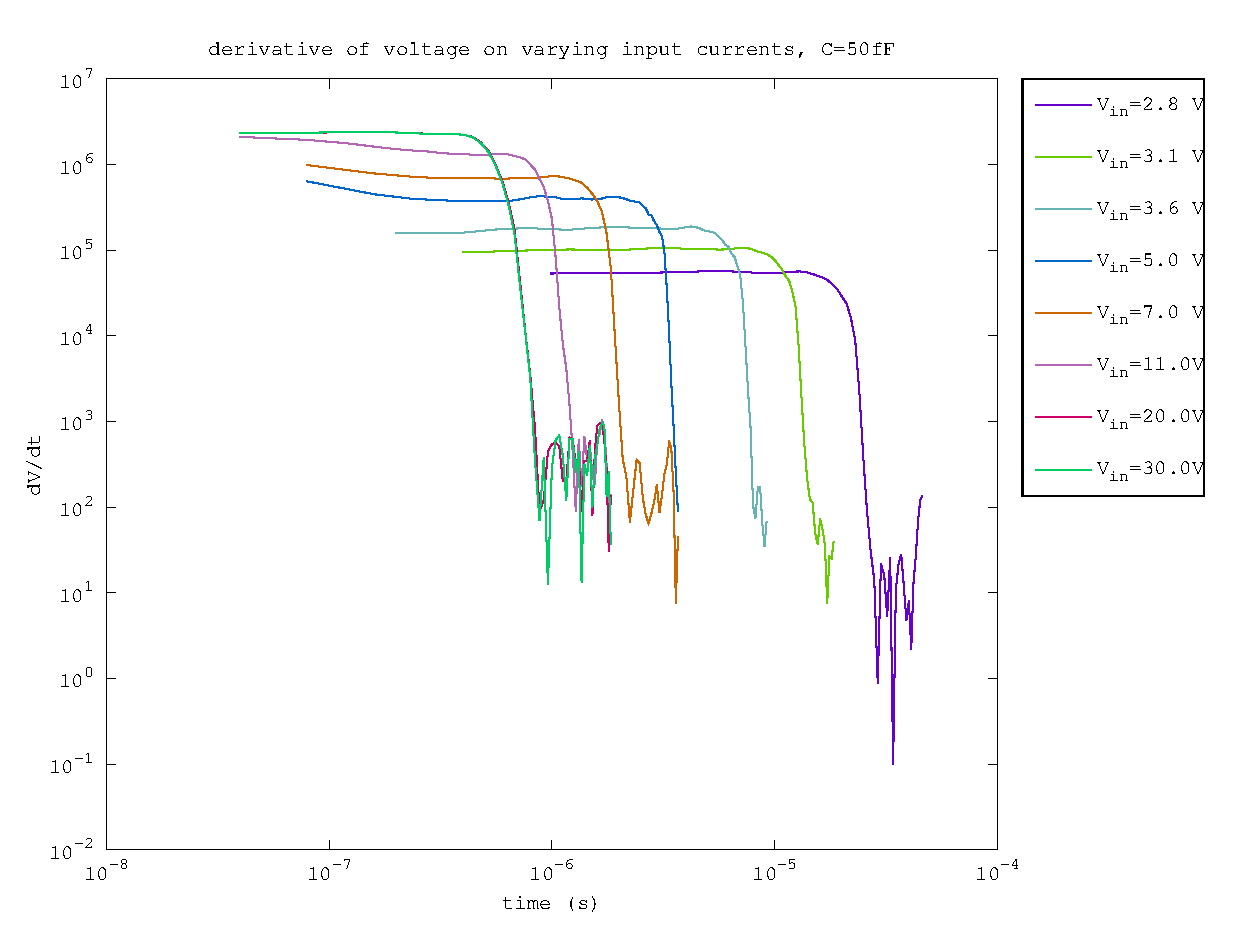
\includegraphics[width=\textwidth]{fig/vbo_d_slope_50fF.eps}
        \caption {$C3$}    
        \label{fig:vbo_d_slopes_50fF}
    \end{subfigure}
    \caption{The plot shows dv/dt against time of the vbo.}
    \label{fig:vbo_d_slopes}
\end{figure}


\Cref{fig:vbo_e_vs_m} shows the $\delta V/\delta t$ against input voltage for VBO across all capacitances. For large voltages seem to behave in a normal linear fashion. The startup shows a scene that looks as if the $C_0$ and $C_1$ setup behave identical, and that the $C_2$ and $C_3$ setup behave identical. This might be due to the lack of measurement points, but is worth investigating further.


\begin{figure}[h]
    \centering
    \includegraphics[width=\textwidth]{fig/vbo_vin_vs_time_sat.eps}
    \caption  {dV/dt of VBO against input voltage for all four capacitances. The x indicate the measurements.}    
    \label{fig:vbo_e_vs_m}
\end{figure}


